\subsubsection{Even Cyclic Extensions}
More care is required to prove Theorem \ref{thm_consistent_cyclic} for even $d$. This difficulty mainly lies in the case when $d$ is only divisible by one odd prime $q$. Consequently, we break down the proof into three distinct cases according to the number of odd prime divisors of $d$. If $d$ has more than one odd prime divisor, then the result follows without much work from Lemma \ref{lem_Cd_odd}, so we prove this first.

\begin{proof}[Proof of Theorem \ref{thm_consistent_cyclic} for even $d$ with more than one odd prime divisor]
    By Remark \ref{rem_radical}, recall that the subgroups present in $\Theta_d$ are precisely those such that $C_k\leq C_{\rad(d)}$, and so following a similar idea to Lemma \ref{lem_Cd_odd}, we define
    $$\mathcal{A}=\{C_k :2\mid k\mid\rad(d)\}\quad\text{and}\quad\mathcal{B}=\{C_k:2\nmid k\mid\rad(d)\},$$
    together with
    $$\Theta_\mathcal{A}=\sum_{H\in\mathcal{A}}\mu(|H|/2)H\quad\text{and}\quad\Theta_\mathcal{B}=\sum_{H\in\mathcal{B}}\mu(|H|)H. $$ 
    For each $k\mid d$, let $L_k=F^{C_{d/k}}$ be the unique subfield of degree $k$ over $K$. The fields $\{F^{C_k}:C_k\in\mathcal{A}\}$ are the intermediate fields of $L_{d/2}/L_{d/\rad(d)}$ and the fields $\{F^{C_k}:C_k\in\mathcal{A}\}$ are the intermediate fields of $F/L_{2d/\rad(d)}$. However, note that 
    $$\Gal(L_{d/2}/L_{d/\rad(d)})=\Gal(F/L_{2d/\rad(d)})=C_{\rad(d)/2},$$
    and by assumption $\rad(d)/2$ is an odd number with more than one prime factor. Then Lemma \ref{lem_subfields} applied to $L_{d/2}/L_{d/\rad(d)}$ and $F/L_{2d/\rad(d)}$ gives $\Theta_\mathcal{A},\Theta_\mathcal{B}\in\QQss$. The calculation in \eqref{eqn_theta} shows that $\Theta_d=\Theta_\mathcal{B}-\Theta_\mathcal{A}$ and therefore 
    $$C(\Theta_d)=\frac{C(\Theta_\mathcal{B})}{C(\Theta_\mathcal{A})}\in\QQss$$
    is the norm of any quadratic extension.
\end{proof}

If $d$ has no odd primes factors, then $d=2^m$ for some $m\geq1$. With the results we have proven in Section {\color{red} Insert here reference when things have been reorganised}, the proof of Theorem \ref{thm_consistent_cyclic} for this case is also fairly straighforward.

\begin{proof}[Proof of Theorem \ref{thm_consistent_cyclic} for $d=2^m$]
    If $d=2^m$, then $\Theta_{d}=C_1-C_2$ and therefore if $L=F^{C_2}$, then 
    $$C(\Theta_{d})=\frac{C_{E/F}}{C_{E/L}}.$$
    %Recall from Lemma \ref{lem_subfields}, that the quadratic subfields of $\QQ(\zeta_{2^m})$ depend on $m=1$, $m=2$ or $m\geq3$, so we consider all three cases. 
    If $m=1$, then $\QQ(\zeta_2)=\QQ$ and there is nothing to prove, so assume that $m\geq2$. As usual, we fix a prime $\pp$ of $K$ of bad reduction and we compute $\Cp(\Theta_d)$. Let $\bar\pp$ be a prime in $L$ above $\pp$. If $\bar\pp$ has multiplicative reduction, then we remark that Table \ref{table_Cp} also applies for $q=2$, and therefore $\Cpb(\Theta_d)$ is a rational square up to factors of $2$. Lemma \ref{lem_subfields} shows that the only subfields of $\QQ(\zeta_{2^m})$ are $\QQ(i),\QQ(\sqrt{2})$ and $\QQ(\sqrt{-2})$, and since
    $$2=\Norm_{\QQ(i)}(1+i)=\Norm_{\QQ(\sqrt{-2})}(2)=\Norm_{\QQ(\sqrt{2})}(2+\sqrt{2}),$$
    it follows that $\Cpb(\Theta_d)$ and hence $\Cpb(\Theta_d)$ are norms from every quadratic subfield of $\QQ(\zeta_{2^m})$.

    Assume now that $\bar\pp$ has additive reduction, let $e_\pp$ and $f_\pp$ be the ramification and inertia degree of $\pp$ over $L$, and note that $e_\pp f_\pp\mid 2^{m-1}$. If $e_\pp f_\pp\neq 2^{m-1}$ then $g_\pp=2^{m-1}/(e_\pp f_\pp)$, the number of primes in $L$ above $\pp$, is even. Since they all have the same local behaviour, it follows that $\Cp(\Theta_d)=\Cpb(\Theta_d)^{g_\pp}\in\QQss$. Hence, we might assume that $e_\pp f_\pp=2^{m-1}$. To compute $\Dp(\Theta_d)$, we note that if $f_\pp\neq 1$, then it is even and hence $N(\bar\pp)=N(\pp)^{f_\pp}\in\QQss$. If $f_\pp=1$, then $e_\pp=2^{m-1}$ and $\pp$ is totally ramified in $L/K$, which is equivalent to being totally ramified in $F/K$. In this case, $\Dp(\Theta_d)$ is a power of $N(\pp)=p^s$ for some rational prime $p$ and $s\geq 1$ and by Propositon \ref{prop_totally_ramified}, it follows that $p^s\equiv 1\pmod{2^m}$. If $s$ is even, then $\Dp(\Theta_d)\in\QQss$ so assume it is odd. If $m=2$, then $p\equiv 1\pmod{4}$ is a norm from $\QQ(i)$ as desired. If $m\geq 3$, then it also follows that $p\equiv 1\pmod{8}$ since $(\ZZ/8\ZZ)^*=C_2\times C_2$. Then
    $$\left(\frac{-1}{p}\right)=\left(\frac{2}{p}\right)=\left(\frac{-2}{p}\right)=1,$$
    so $p$ splits in $\QQ(i),\QQ(\sqrt{2})$ and $\QQ(\sqrt{-2})$. Since they all have class number $1$, $p$ is a norm from all of them, as desired.

    Finally, we compute $\Tp(\Theta_d)$. Since $2$ is a norm of $\QQ(i),\QQ(\sqrt{2})$ and $\QQ(\sqrt{-2})$, we only need to control the contribution of $3$. Under the assumption that $e_\pp f_\pp=2^{m-1}$, $\bar\pp$ is either inert or ramifies in $F/L$, but it can never split. If $n=\nu_{\bar\pp}(\Delta_{E,\bar\pp}^{\min})$, we can see from Lemma \ref{lem_add_tam} that a factor of $3$ can only arise if $E$ has potentially good reduction at $\bar\pp$, $\gcd(n,12)=2$ and $\bar\pp$ ramifies in $L/K$, so assume this is the case. Then let $L'=F^{C_4}$ and $\pp'=\bar\pp\cap L'$, and note that $E$ has additive reduction at $\pp'$. If $e_\pp\geq 2$, then $\pp'$ ramifies in $L/L'$ and the valuation of the minimal discriminant at $\pp'$ is either $n/2$ or $(n+12)/2$. In either case, $\gcd(\nu_{\pp'}(\Delta_{E,\pp'}^{\min}),12)=1$, a contradiction. Hence, $e_\pp=1$ and therefore $\pp'$ is inert in $L/L'$. But then we are precisely under the conditions of Lemma \ref{lem_notthree}, which implies that $\sqrt{B}\not\in F_\fP$, where $\fP$ is the unique prime in $F$ above $\bar\pp$. Hence, $c_\fP(E/F)=1$ and hence $\Tp(\Theta_d)\in\QQss$. We have covered all cases, and the result follows.
\end{proof}

The remaining of this section is therefore devoted to the case when $d$ is divisible by one odd prime $q$, so $d=2^mq^n$. 
%When $d$ has this form, then $\Theta_d=C_1-C_2-C_q+C_{2q}$ and therefore fix $\Theta_d$ to have this expression for the remaining of this section. 
Recall that the quadratic subfields of $\QQ(\zeta_{2^mq^n})$ depend on whether $m=1$, $m=2$ or $m\geq 3$. Consequently, we prove three results that will be essential to prove the general version of each different case. The first covers the case $m=1$.

\begin{lemma}\label{lem_C2p}
    Let $q$ be an odd prime and let $F/K$ be a Galois extension of number fields such that $\Gal(F/K)=C_{2q}$ and let $L_k=F^{C_{2q/k}}$ be the intermediate fields such that $[L_k:K]=k$. Let $E/\QQ$ be an elliptic curve and let $\Theta_{2q}=C_{2q}-C_q-C_2+C_1\in B(C_{2q})$. Then
    $$C(\Theta_{2q})=\frac{C_{E/F}C_{E/K}}{C_{E/L_2}C_{E/L_q}}$$
    is a norm from $\QQ(\sqrt{q^*})$.
\end{lemma}

\begin{proof}
    Similarly to the proofs of Lemma \ref{lem_Cp} and \ref{lem_Cpq}, let $\pp$ be a prime in $K$ and assume that $\Delta_E=\Delta_{E,\pp}^{\min}$. The splitting behaviour of a prime $\pp$ in $K$ is again determined by $e_\pp$ and $f_\pp$ and therefore if $\pp$ has multiplicative reduction $\Dp(\Theta_{2q})=1$ and the following table records $\Tp(\Theta_{2q})$.

    \begin{table}[!ht]
        \centering
        \begin{tabular}{|l|l|l|l|l|l|l|}
        \hline
        $e_\pp$ & $f_\pp$  & $\Tp(C_{2q})$ & $\Tp(C_2)$ & $\Tp(C_q)$ & $\Tp(C_1)$ & $\Tp(\Theta_{2q})$ \\ \hline
        $1$ & $1$ & $n;\tilde{n}$ & $n^q;\tilde{n}^q$ & $n^2;\tilde{n}^2$ & $n^{2q};\tilde{n}^{2q}$ & $\square$ \\ \hline
        $1$ & $q$ & $n;\tilde{n}$ & $n;\tilde{n}$ & $n^2;\tilde{n}^2$ & $n^2;\tilde{n}^2$ & $\square$ \\ \hline
        $1$ & $2$ & $n;\tilde{n}$ & $n^q;\tilde{n}^q$ & $n;n$ & $n^q;n^q$ & $\square$ \\ \hline
        $1$ & $2q$ & $n;\tilde{n}$ & $n;\tilde{n}$ & $n;n$ & $n;n$ & $\square$ \\ \hline
        $q$ & $1$ & $n;\tilde{n}$ & $qn;\tilde{n}$ & $n^2;\tilde{n}^2$ & $q^2n^2;\tilde{n}^2$ & $q\square;\square$ \\ \hline
        $q$ & $2$ & $n;\tilde{n}$ & $qn;\tilde{n}$ & $n;n$ & $qn;n$ & $\square$ \\ \hline
        $2$ & $1$ & $n;\tilde{n}$ & $n^q;\tilde{n}^q$ & $2n;1$ & $2^qn^q;1^q$ & $\square$ \\ \hline
        $2$ & $q$ & $n;\tilde{n}$ & $n;\tilde{n}$ & $2n;1$ & $2n;1$ & $\square$ \\ \hline
        $2q$ & $1$ & $n;\tilde{n}$ & $qn;\tilde{n}$ & $2n;1$ & $2qn;1$ & $\square$ \\ \hline
        \end{tabular}
        \caption{Contribution of multiplicative reduction primes in a $C_{2q}$ extension.}
    \end{table}

    Since $q$ is a norm from $\QQ(\sqrt{q^*})$, then $\Tp(\Theta_{2q})$ is also a norm. Now assume that $\pp$ has additive reduction and let $p\ZZ=\pp\cap\QQ$. We first consider the contribution of the Tamagawa numbers. Note that $L_q/K$ and $F/L_2$ are $C_q$ extensions and therefore $\Tp(\Theta_{2q})\in\QQss$ if $q\neq 3$ and a square up to factors of $3$ if $q=3$. In either case, $\Tp(\Theta_{2q})$ is a norm from $\QQ(\sqrt{q^*})$.

    Finally, to compute $\Dp(\Theta_{2q})$, let $n=\nu_\pp(\Delta_{E,\pp}^{\min})$ and note that all terms cancel unless $\pp$ ramifies in $F$. If $e_\pp=2$, then
    \begin{equation}\label{eqn_ep=2}
        \Dp(C_{2q})=\Dp(C_2)=1,\quad \Dp(C_q)=N(\pp)^{\floor{\frac{2n}{12}}}\quad\text{and}\quad \Dp(C_1)=N(\pp)^{q\floor{\frac{2n}{12}}},
    \end{equation}
    and therefore $D(\Theta_{2q})=N(\pp)^{(q-1)\floor{n/6}}\in\QQss$, a rational square. If $q\mid e_\pp$, then $q\mid N(\pp)-1$ by Proposition \ref{prop_totally_ramified}, and the reasoning is now identical to Lemma \ref{lem_Cp}. Write $N(\pp)=p^s$ for some $s\geq1$ and note that $\Dp(\Theta_{2q})\in\QQss$ if $s$ is even. Hence, we assume that $s$ is odd. In this case, $p=q$ if $(L_q)_\fP/K_\pp$ is wildly ramified and $p$ splits in $\QQ(q^*)$ if $(L_q)_\fP/K_\pp$ is tamely ramified. In either case, by Corollaries \ref{p-norm} and \ref{cor_psplit_pnorm}, $p$ is a norm from $\QQ(\sqrt{q^*})$, and hence so is $\Dp(\Theta_{2q})$.
    The result follows again from \eqref{eqn_local_contr}.
\end{proof}

Following this, we state and prove the analogous result for $m=2$.

\begin{lemma}\label{lem_C4p}
    Let $q$ be an odd prime and let $F/K$ be a Galois extension of number fields such that $\Gal(F/K)=C_{4q}$ and let $L_k=F^{C_{4q/k}}$ be the intermediate fields such that $[L_k:K]=k$. Let $E/\QQ$ be an elliptic curve with semistable reduction at $2$ and $3$ and let $\Theta_{4q}=C_1-C_2-C_q+C_{2q}$. Then 
    $$C(\Theta_{4q})=\frac{C_{E/F}C_{E/L_2}}{C_{E/L_4}C_{E/L_{2q}}}$$
    is a norm from $\QQ(i),\QQ(\sqrt{q})$ and $\QQ(\sqrt{-q})$. Moreover, $\Tp(\Theta_{4q})\in\QQss$ for any prime $\pp$ in $K$, and $\Dp(\Theta_{4q})\in\QQss$ unless $E$ has additive reduction at $\pp$ and $\pp$ is totally ramified in $F/K$.
\end{lemma}

\begin{proof}
    All fields appearing in the product are intermediate fields of $F/L_2$, and $\Gal(F/L_2)=C_{2q}$. Let $\pp$ be a prime in $K$, let $\bar\pp\mid\pp$ be a prime above $\pp$ in $L_2$ and let $p\ZZ=\pp\cap\QQ$. Assume also that $\Delta_E=\Delta_{E,\pp}^{\min}$. Lemma \ref{lem_C2p} shows that if $E$ has multiplicative reduction over $\bar\pp$, $C_{\fP\mid\bar\pp}(\Theta_{4q})\in\QQss$ unless $e_{\bar\pp}=q$ and $f_{\bar\pp}=1$ over $F$. When this holds, $\bar\pp$ ramifies in $L_{2q}/L_2$ and is split in $L_4/L_2$, and this forces $\pp$ to split in $L_2/K$ too. Hence, $\pp=\bar\pp\bar\pp'$ for two \textbf{distinct} primes in $K$ that have the same local behaviour and therefore $\Cp(\Theta_{4q})=C_{\fP\mid\bar\pp}(\Theta_{4q})C_{\fP\mid\bar\pp'}(\Theta_{4q})=C_{\fP\mid\bar\pp}(\Theta_{4q})^2\in\QQss$, as desired.

    \begin{figure}[!ht]
        \centering
        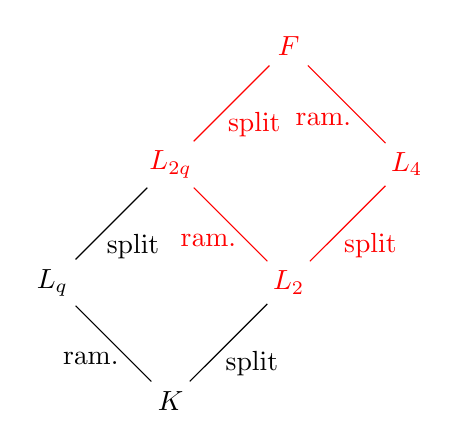
\begin{tikzpicture}

            \node (Q1) at (0,0) {$K$};
            \node (Q2) at (-1.5,1.5) {$L_q$};
            \node [red] (Q3) at (3,3) {$L_4$};
            \node [red] (Q4) at (1.5,1.5) {$L_2$};
            \node [red] (Q5) at (1.5,4.5) {$F$};
            \node [red] (Q6) at (0,3) {$L_{2q}$};
            

            \draw (Q1)--(Q2) node [pos=0.8, below,inner sep=0.4cm] {ram.};
            \draw (Q1)--(Q4) node [pos=0.8, below,inner sep=0.4cm] {split};
            \draw (Q2)--(Q6) node [pos=0.8, below,inner sep=0.4cm] {split};
            \draw [red] (Q3)--(Q5) node [pos=0.8, below,inner sep=0.4cm] {ram.};
            \draw [red] (Q4)--(Q6) node [pos=0.8, below,inner sep=0.4cm] {ram.};
            \draw [red] (Q6)--(Q5) node [pos=0.8, below,inner sep=0.4cm] {split};
            \draw [red] (Q4)--(Q3) node [pos=0.8, below,inner sep=0.4cm] {split};
        \end{tikzpicture}
        \caption[short]{\centering Field diagram for a $C_{4q}$ extension, together with the splitting\newline behaviour of a prime $\pp$ in $L_2$ with $e_\pp=q$ and $f_\pp=1$ over $F$.}
    \end{figure}

    Assume now that $E$ has additive reduction over $\bar\pp$. When $q=3$, controlling the Tamagawa numbers is lengthy, so we leave it for the end. We calculate first $\Dp(\Theta_{4q})$, which is $1$ unless $\bar\pp$ ramifies in $L/F_2$ (equivalently, $\pp$ ramifies in $L/K$). If $\pp$ is inert in $L_2/K$, then $N(\bar{\pp})\in\QQss$ and hence the size of all residues fields above $\pp$ are also squares and consequently $\Dp(\Theta_{4q})\in\QQss$ using Lemma \ref{lem_Dterms}. If $\pp=\bar\pp\bar\pp'$ splits, then $D_{\fP\mid\bar\fp}(\Theta_{4q})=D_{\fP\mid\bar\fp'}(\Theta_{4q})$, and therefore $\Dp(\Theta_{4_q})\in\QQss$ too. Finally, assume that $\pp=\bar\pp^2$ ramifies in $L_2/K$, which implies that $\bar\fp$ also ramifies in $L_4/L_2$. On the other hand, if $\bar\pp$ is unramified at $L_{2q}/L_2$, \eqref{eqn_ep=2} during the proof of Lemma \ref{lem_C2p} shows that $\Dp(\Theta_{4q})\in\QQss$ too. 

    We are therefore left with the case where $\pp$ is totally ramified in $F/K$, and Proposition \ref{prop_totally_ramified} implies that $4q\mid N(\pp)-1$. If we let $n=\nu_{\pp}(\Delta_{E,\pp}^{\min})$, Lemma \ref{lem_Dterms} implies that 
    \begin{equation*}\label{eqn_DtermsC4p}
        \Dp(\Theta_{4q})=N(\pp)^{\floor{\frac{n}{6}}-\floor{\frac{n}{3}}-\floor{\frac{qn}{6}}+\floor{\frac{qn}{3}}}.
    \end{equation*}
    Again, the parity of the expression only depends on $q,n\pmod{12}$. One can easily check that for $n\in\{2,3,4,6,8,9,10\}$ and $q\in\{1,5,7,11\}$, the above expression is a square unless $q\equiv 3\pmod{4}$ and $n$ is odd, so we assume this is the case. Write $N(\pp)=p^s$ for some $s\geq1$, which satisfies $p^s\equiv1\pmod{4q}$. If $s$ is even, then $\Dp(\Theta_{4q})\in\QQss$, so assume that $s$ is odd. Since $p^s\equiv1\pmod{4}$, this implies that $p\equiv1\pmod{4}$ and hence $p$ is a norm from $\QQ(i)$, which implies that $\Dp(\Theta_{4q})$ is a norm from $\QQ(i)$ too. Furthermore, the fact that $p^s\equiv1\pmod{4q}$ implies that
    $$\left(\frac{-q}{p}\right)=\left(\frac{q}{p}\right)=\left(\frac{p}{q}\right)=\left(\frac{p^s}{q}\right)=1,$$
    and therefore $p$ splits both in $\QQ(\sqrt{q})$ and $\QQ(\sqrt{-q})$. Since $q\equiv3\pmod{4}$, both fields have odd class number (Theorem \ref{thm_class_number}), and hence $p$ and $\Dp(\Theta_{4q})$ are norms from $\QQ(\sqrt{q})$ and $\QQ(\sqrt{-q})$ as desired. 

    Finally, we discuss Tamagawa numbers. Note that $L_{2q}/L_2$ and $F/L_4$ are $C_q$ extensions and therefore by Lemma \ref{lem_Cp} it follows that $\Dp(\Theta_{4q})\in\QQss$ if $q\neq3$. If $q=3$, it is also the case that $\Dp(\Theta_{4q})\in\QQss$, but more work is required. We prove this as a separate lemma, from which the result follows.    
\end{proof}

\begin{lemma}
    Let $L/K$ be a Galois extension of number fields with $\Gal(L/K)=C_{12}$ and let $L_k=F^{C_{12/k}}$ be the intermediate fields such that $[L_k:K]=k$. Let $E/\QQ$ be an elliptic curve and let $\pp$ be a prime in $K$ not dividing $2$ or $3$ such that $E$ has potentially good reduction at $\pp$. If $\Theta_{12}=C_1-C_2-C_3+C_6\in B(C_{12})$, then $$\Tp(\Theta_{12})=\frac{\Tp(E/F)\Tp(E/L_2)}{\Tp(E/L_6)\Tp(E/L_4)}\in\QQss.$$
\end{lemma}
\begin{proof}
    Let $\bar\pp$ be a prime in $L_2$ above $\pp$ and let $n=\nu_{\bar\pp}(\Delta_{E,\bar\pp}^{\min})$ be the minimal discriminant of $E$ at $\bar\pp$. If $\pp$ is unramified in $L_3/K$, then so is $\bar\pp$ in $L_6/L_2$ and the primes above them in $F/L_4$. From Lemma \ref{lem_Cp}, we know that that the product of Tamagawa numbers in unramified $C_3$ extensions is a square, so assume that $\pp$ ramifies in $L_3/K$.

    The proof is now divided in three cases, depending on the splitting behaviour of $\pp$ in $L_2$. If $\pp$ splits in $L_2/K$, then $\pp=\bar\pp\bar\pp'$ where $\bar\pp$ and $\bar\pp'$ have the same local behaviour. Therefore, $T_{\fP\mid\pp}(\Theta_{12})=T_{\fP\mid\bar\pp}(\Theta_{12})T_{\fP\mid\bar\pp'}(\Theta_{12})\in\QQss$. 
    
    Next, suppose that $\pp$ is inert in $L_2/K$, which implies that $\bar\pp$ is either inert or ramified in $L_4/L_2$. Let $\fP$ be the prime in $L_4$ above $\bar\pp$. If $\bar\pp$ is inert in $L_4/L_2$, then the valuation of the minimal discriminant of $E$ at $\fP$ is also $n$ and the splitting behaviour of $\bar\pp$ in $L_6/L_2$ coincides with the splitting behaviour of $\fP$ in $F/L_4$. Hence, 
    $$\frac{\Tp(E/F)}{\Tp(E/L_4)}=\frac{\Tp(E/L_6)}{\Tp(E/L_2)},$$
    and therefore $\Tp(\Theta_{12})=1$. The case where $\bar\pp$ is ramified in $L_4/L_2$ is more subtle. We have already seen that in ramified $C_3$ extensions we cannot obtain factors of $2$. Upon inspection of Lemma \ref{lem_add_tam}, one can easily show that the Tamagawa numbers cancel out if $\gcd(n,12)\in\{3,4,6,12\}$, so we only need to consider the case $\gcd(n,12)=2$. Since $\Gal((L_4)_\fP/K_\pp)=C_4$ and $e_{\fP\mid\pp}=f_{\fP\mid\pp}=2$, Lemma \ref{lem_notthree} shows that $\sqrt{B}\not\in F_{\fP}$ and therefore $c_\fP(E/F)=1$, which imples that $\Dp(\Theta_{12})\in\QQss$.

    Finally, assume that $\pp$ ramifies in $L_2/K$ so that $\pp=\bar\pp^2$. This immediately implies that $\bar\pp$ also ramifies in $L_4/L_2$, and therefore $\pp$ is totally ramified in $F/K$. As mentioned above, the Tamagawa numbers cancel unless $\gcd(n,12)=2$. However, recall that $E$ has potentially good reduction at $\pp$, and since $\pp=\bar\pp^2$ ramifies, then the valuation of the minimal discriminant at $\pp$ is $n/2$ or $(n+12)/2$. But then $\gcd(\nu_\pp(\Delta_{E,\pp}^{\min}),12)=\gcd(n/2,12)=1$, a contradiction. Hence, $\Tp(\Theta_{12})\in\QQss$ as desired.
\end{proof}

Finally, we state and prove the last result, from which the case $m\geq3$ follows easily. One needs to check that the product of local factors is the norm of many quadratic subfields; thankfully, Lemma \ref{lem_C4p} has done most of work required.

\begin{lemma}\label{lem_C8p}
    Let $q$ be an odd prime and let $F/K$ be a Galois extension of number fields such that $\Gal(F/K)=C_{8q}$ and let $L_k=F^{C_{8q/k}}$ be the intermediate fields such that $[L_k:K]=k$. Let $E/\QQ$ be an elliptic curve with semistable reduction at $2$ and $3$ and let $\Theta_{8q}=C_1-C_2-C_q+C_{2q}$. Then 
    $$C(\Theta_{8q})=\frac{C_{E/F}C_{E/L_4}}{C_{E/L_8}C_{E/L_{4q}}}\in\QQss.$$
    %is a norm from $\QQ(\sqrt{D})$ for each $D\in\{-1,\pm2,\pm q,\pm 2q\}$.
\end{lemma}

\begin{proof}
    We prove the result locally for all primes in $L_2$, and note $\Gal(F/L_2)=4q$. Let $\bar\pp$ and assume that $\Delta_E=\Delta_{E,\bar\pp}^{\min}$. Since the relation $\Theta_{4q}=C_1-C_2-C_q+C_{2q}\in B(C_{4q})$ has the same fixed fields as $\Theta_{8q}$, by Lemma \ref{lem_C4p}, we know that $\Tpb(\Theta_{8q})\in\QQss$ for any $\bar\pp$ and $\Dpb(\Theta_{8q})\in\QQss$ too unless $\bar\pp$ is totally ramified in $F/L_2$ and $E$ has potentially good reduction at $\bar\pp$, so assume this is the case. If $\pp=\bar\pp\cap K$, then it also follows that $\pp$ is totally ramified in $F/K$ and $E$ has potentially good reduction at $\pp$. If $n=\nu_{\bar\pp}(\Delta_{E,\bar\pp}^{\min})$, then recall from Lemma \ref{lem_C4p} that 
    $$\Dpb(\Theta_{8q})=N(\bar\pp)^{\floor{\frac{n}{6}}-\floor{\frac{n}{3}}-\floor{\frac{qn}{6}}+\floor{\frac{qn}{3}}},$$
    and that the exponent is even unless $n$ is odd and $q\equiv 3\pmod{4}$. However, $\pp=\bar\pp^2$ is ramified in $L_2/K$ and therefore $n\equiv 2\nu_\pp(\Delta_{E,\pp}^{\min})\pmod{12}$. That is, $n$ is even and therefore $\Dpb(\Theta_{8q})\in\QQss$ as desired.
\end{proof}
%%% THIS IS ALL PROBABLY NOT NEEDED NOW
%Again, $\Dp(\Theta_{8q})$ does not change up to squares if $\Delta_{E}$ is reescaled so assume that $\Delta_{E}=\Delta_{E,\pp}^{\min}$. Under these assumptions, $\Dpb(\Theta_{8q})=\Dp(\Theta_{8q})$ is a power of $N(\pp)=N(\bar\pp)=p^s$ for some rational prime $p$ and $s\geq1$. If $s$ is even, then $\Dpb(\Theta_{8q})\in\QQss$, so assume that $s$ is odd. In addition, by Proposition \ref{prop_totally_ramified}, it follows that $p^s\equiv 1\pmod{8q}$. Since $s$ is odd and $(\ZZ/8\ZZ)^*=C_2\times C_2$, it follows that $p\equiv 1\pmod{8}$ and therefore
%\begin{equation}\label{eqn_psplitsin2}
%    \left(\frac{-1}{p}\right)=\left(\frac{2}{p}\right)=\left(\frac{-2}{p}\right)=1.
%\end{equation}
%Furthermore, since $p^s\equiv1\pmod{8s}$ and $s$ is odd, then 
%\begin{equation}\label{eqn_psplitsinq}
%    \left(\frac{-q}{p}\right)=\left(\frac{q}{p}\right)=\left(\frac{p}{q}\right)=1.
%\end{equation}
%Combining \eqref{eqn_psplitsin2} and \eqref{eqn_psplitsinq} together with multiplicativity of the Legendre symbol, it follows that $p$ splits in every quadratic subfield $\QQ(\sqrt{D})$ for $D\in\{-1,\pm2,\pm q,\pm2q\}$.


We are now ready to prove the remaining case of Theorem \ref{thm_consistent_cyclic}.

\begin{proof}[Proof of Theorem \ref{thm_consistent_cyclic} for $d$ even and with one odd prime factor.]
    In this case, write $d=2^mq^n$ for $n,m\geq 1$ and note that $\Theta_{d}=C_1-C_2-C_q+C_{2q}$ is the $\psi_d$-relation of a faithful character of $C_d$. If $m=1$, Lemma \ref{lem_C2p} applied to the $C_{2q}$ extension $F/F^{C_{2q}}$ shows that $C(\Theta_d)$ is a norm from $\QQ(\sqrt{q^*})$, which is the only subfield of $\QQ(\zeta_{2q^n})$ by Lemma \ref{lem_subfields}. If $m=2$, then Lemma \ref{lem_C4p} applied to the $C_{4q}$ extension $F/F^{C_{4q}}$ shows that $C(\Theta_{d})$ is a norm from $\QQ(i),\QQ(\sqrt{q})$ and $\QQ(\sqrt{-q})$, which are all quadratic subfields of $\QQ(\zeta_{4q^n})$. Finally, if $m\geq3$, Lemma \ref{lem_C8p} applied to $F/F^{C_{8q}}$ shows that $C(\Theta_{8q})\in\QQss$, which is the norm from any quadratic subfield. The result follows.
\end{proof}

